\section{Map-Reduce Pipelines}
Large-scale data-parallel computation is increasingly important.  Technologies such as FlumeJava, have addressed the difficulty of maximizing computational power for kinds of workloads~\cite{pldi:flumejava}.  However, debugging these programs remains difficult, particularly in the presence of errors in giga-, tera-, and peta-scale inputs.  For example, the presence of a single unexpected zero value can dramatically alter the result of many mathematical programs.  Finding and correcting these errors, preferably automatically, is an important step in making large-scale computation more robust.

\begin{figure*}[t]
	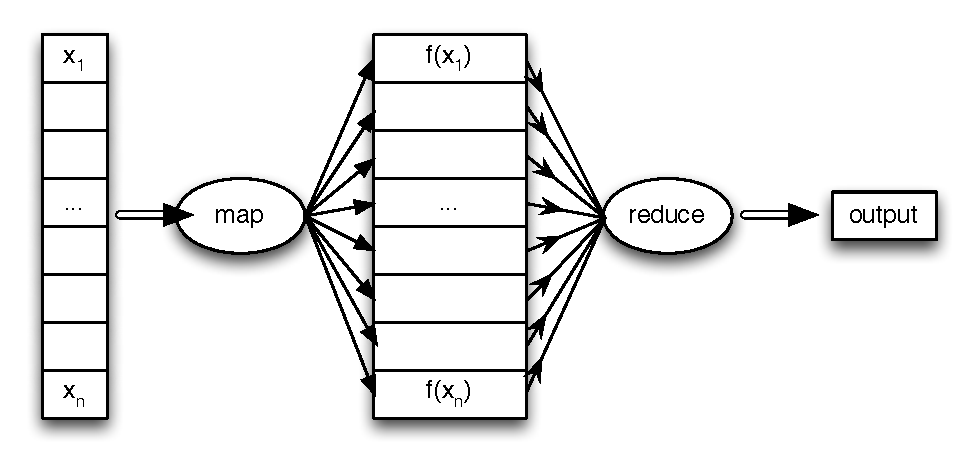
\includegraphics[width=2.5in]{images/mapreduce}
  % \hspace{30px}
  \hfill
	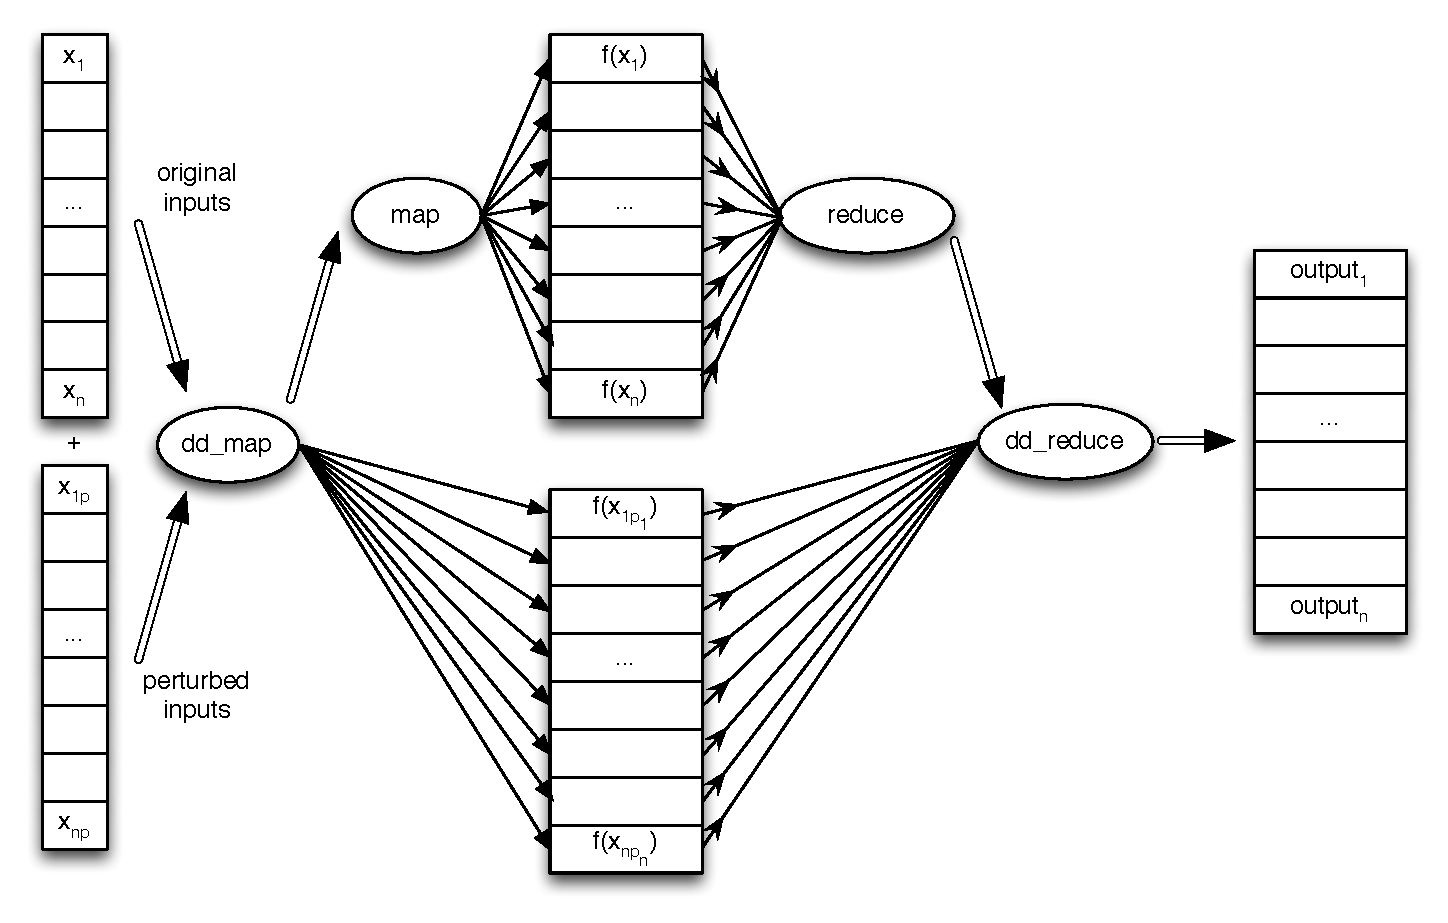
\includegraphics[width=3.25in]{images/mapreduce_dd}
	\caption{
		On the left, a typical MapReduce job.  On the right, a data-debug-augmented MapReduce job.  Each additional output is a version of the computation with the unusually-impactful values automatically excluded.\label{fig:mapreduce_pipeline}
	}
\end{figure*}

Data-parallel programs share many of the same properties that make data-debugging a useful technique.  The input to the mapper stage of a MapReduce problem is a large, homogenous vector amenable to the same kind of input perturbation that \checkcell{} uses.  A key property of the computation kernel in a MapReduce job is that code be re-entrant, thus data-debugging can be inserted into a MapReduce job without affecting the semantics of the original program.

MapReduce and Hadoop jobs themselves are low-level, but frameworks like FlumeJava (and by extension, its Hadoop dual, Crunch) represent multi-stage MapReduce programs by their dependency graph.  This high-level representation gives the runtime global information that facilitates performance-enhancing program transformations, such as reordering of functions in the program call graph.

As with \checkcell, data-debugging functions can transparently augment a FlumeJava program.  The tradeoff, which we seek to minimize, is a small performance penalty for the additional robustness data-debugging provides. Data-debugging techniques can be piggybacked on this high-level representation so that impact analysis can take advantage of underutilized parallelism to minimize the performance impact of our technique.

A high-level dependency analysis allows at least two kinds of program transformations to facilitate data-debugging at scale.  First, a data-debugging-enhanced FlumeJava would augment the map stage with perturbed input values to be computed in parallel, and the reducer function would be augmented with the impact computation.  Our implementation of \checkcell relies on Microsoft Excel's ability to recognize when partial recomputation of the dependency graph is possible, for efficiency purposes.  Thus, second, a data-debugging-enhanced FlumeJava runtime would both need to recognize when an impact calculation may be performed for only a subset of the program dependency graph and when the dependency analysis itself contains overlapping subproblems which may be memoized for performance purposes.

Once impact scores are known for a set of MapReduce program inputs, the data-debug runtime can be instructed to re-run the computation with the unusually-impactful inputs either removed or replaced with user-specfied values.  The degree of unusualness, in terms of standard deviations from the norm, may be used to control the degree of \emph{input trimming} performed on the MapReduce input vector.  Again, a high-level representation of the program graph allows this recomputation to be performed for the minimum cost possible.